\documentclass{article}
\usepackage[spanish]{babel}
	\deactivatetilden
\spanishdecimal{.}
\addto\captionsspanish{\def\tablename{Tabla}}
\addto\captionsspanish{\def\listtablename{\'Indice de tablas}}
\usepackage[numbers,sort&compress]{natbib}
\usepackage[T1]{fontenc}
\usepackage[utf8]{inputenc}
\usepackage{graphicx}
\usepackage{url}
\usepackage{graphicx}
\graphicspath{{Figuras/}}
\usepackage[numbers,sort&compress]{natbib}
\usepackage[clearempty,pagestyles]{titlesec}
\usepackage{anysize}
\usepackage{xcolor, colortbl}
\usepackage{array, multirow, multicol}
\usepackage{enumerate} 

\def\baselinestretch{1.5}
\papersize{27.9cm}{21.5cm} 
\marginsize{2cm}{2cm}{1cm}{1cm}

\title {Frentes de Pareto Genético}
\author{Julio Garc\'ia}
\pagestyle{empty}

\pagestyle{empty}
\begin{document}
	\renewcommand{\listtablename}{Índice de tablas}
	\renewcommand{\tablename}{Cuadro}
	\maketitle
	
	\section{Introducción}
	En el presente trabajo se busca como objetivo principal el estudio de las soluciones no dominadas en la optimización multicriterio, en otras palabras, se estudiarán los frentes de Pareto para múltiples criterios.\\
	La optimización multicriterio es sumamente importante para la industria, normalmente las áreas de una misma empresa tienen diferentes criterios, y por lo regular están encontrados, entre ellos son: minimizar costos de producción, maximizar cobertura, minimizar costros de transporte entre otros. Sin embargo, cada uno de ellos es importante para la Dirección y cumplimiento de objetivos, es ahí donde se vuelve relevante el estudio de esta área. En este trabajo se busca analizar la relación que se tiene entre las soluciones de un frente de Pareto, el porcentaje de soluciones que dominan y la cantidad de criterios. 

	
	\section{Desarrollo}
	En este trabajo se analiza la relación del porcentaje de soluciones de Pareto como función del número de funciones objetivo, el cuál varía de dos a doce objetivos. Para este estudio se realizarán diagramas de caja-bigote y analizaremos si es que existen diferencias significativas en los datos.\\
	En base a la tarea propuesto por la Dra. Shaffer \cite{pa}, se tomó de referencia para ajustar la cantidad de objetivos a mostrar y cambiar la métrica deseada. El código propuesto es basado en el de la Dra. Shaffer \cite{pa1}, se añadió la métrica a calcular (porcentaje de soluciones de Pareto), se agregó un ciclo para realizar una cantidad de repeticiones por objetivo y se ajustaron las gráficas de acuerdo a lo solicitado.\\


	\section{Experimentación y resultados}
	En esta sección se describe el ambiente computacional y los resultados obtenidos con la simulación. El código de dicha simulación fue realizado en el lenguaje computacional Python por ser más simple el código. Las características del equipo computacional son:  procesador 1 Intel Core i7, con memoria RAM de 16GB y hasta 8 núcleos de procesamiento. Dicho código fue incorporado en el repositorio \cite{p_a}.\\ 
	A continuación, se muestra los resultados obtenidos en la simulación en la tabla 1 Resultados de experimentación, además, se muestra dichos resultados en el gráfico 1 Diagrama de Violín y de Caja Bigote.\\  
	La experimentación consiste en realizar 15 réplicas para cada cantidad de objetivos, variando los objetivos de 2 a 12.  Los valores de los resultados se encuentran entre cero y uno, cuando se aproximan a cero, indica que se tienen menos cantidad de soluciones no dominadas, mientras los valores se acercan a uno, indica que se tiene mayor cantidad de soluciones no dominadas.\\
	\newpage

	
\begin{table}[h!]
	\centering
	
	\caption{Resultados  de $2$ a $12$ funciones con  $15$ replicas}
	\begin{tabular}{|c|c|c|c|c|c|c|c|c|c|c|c|}
		\hline
		\rowcolor[rgb]{ .706,  .776,  .906}       & \multicolumn{11}{c|}{Criterios} \\
		\hline
		\rowcolor[rgb]{ .906,  .902,  .902} \multicolumn{1}{|c|}{Replica } & \multicolumn{1}{c|}{dos} & \multicolumn{1}{c|}{tres} & \multicolumn{1}{c|}{cuatro} & \multicolumn{1}{c|}{cinco} & \multicolumn{1}{c|}{seis} & \multicolumn{1}{c|}{siete} & \multicolumn{1}{c|}{ocho} & \multicolumn{1}{c|}{nueve} & \multicolumn{1}{c|}{diez} & \multicolumn{1}{c|}{once} & \multicolumn{1}{c|}{doce} \\
		\hline
		\rowcolor[rgb]{ .906,  .902,  .902} \multicolumn{1}{|r|}{1} & \cellcolor[rgb]{ 1,  1,  1}0.004 & \cellcolor[rgb]{ 1,  1,  1}0.068 & \cellcolor[rgb]{ 1,  1,  1}0.220 & \cellcolor[rgb]{ 1,  1,  1}0.580 & \cellcolor[rgb]{ 1,  1,  1}0.888 & \cellcolor[rgb]{ 1,  1,  1}1.000 & \cellcolor[rgb]{ 1,  1,  1}0.992 & \cellcolor[rgb]{ 1,  1,  1}0.920 & \cellcolor[rgb]{ 1,  1,  1}0.888 & \cellcolor[rgb]{ 1,  1,  1}0.996 & \cellcolor[rgb]{ 1,  1,  1}1.000 \\
		\hline
		\rowcolor[rgb]{ .906,  .902,  .902} \multicolumn{1}{|r|}{2} & \cellcolor[rgb]{ 1,  1,  1}0.032 & \cellcolor[rgb]{ 1,  1,  1}0.056 & \cellcolor[rgb]{ 1,  1,  1}0.372 & \cellcolor[rgb]{ 1,  1,  1}0.020 & \cellcolor[rgb]{ 1,  1,  1}0.836 & \cellcolor[rgb]{ 1,  1,  1}0.960& \cellcolor[rgb]{ 1,  1,  1}0.996 & \cellcolor[rgb]{ 1,  1,  1}0.992 & \cellcolor[rgb]{ 1,  1,  1}1.000 & \cellcolor[rgb]{ 1,  1,  1}1.000 & \cellcolor[rgb]{ 1,  1,  1}1.000 \\
		\hline
		\rowcolor[rgb]{ .906,  .902,  .902} \multicolumn{1}{|r|}{3} & \cellcolor[rgb]{ 1,  1,  1}0.004 & \cellcolor[rgb]{ 1,  1,  1}0.084 & \cellcolor[rgb]{ 1,  1,  1}0.580 & \cellcolor[rgb]{ 1,  1,  1}0.168 & \cellcolor[rgb]{ 1,  1,  1}0.504 & \cellcolor[rgb]{ 1,  1,  1}1.000 & \cellcolor[rgb]{ 1,  1,  1}1.000 & \cellcolor[rgb]{ 1,  1,  1}1.000 & \cellcolor[rgb]{ 1,  1,  1}0.976 & \cellcolor[rgb]{ 1,  1,  1}1.000 & \cellcolor[rgb]{ 1,  1,  1}1.000 \\
		\hline
		\rowcolor[rgb]{ .906,  .902,  .902} \multicolumn{1}{|r|}{4} & \cellcolor[rgb]{ 1,  1,  1}0.048 & \cellcolor[rgb]{ 1,  1,  1}0.156 & \cellcolor[rgb]{ 1,  1,  1}0.288 & \cellcolor[rgb]{ 1,  1,  1}0.196 & \cellcolor[rgb]{ 1,  1,  1}0.952 & \cellcolor[rgb]{ 1,  1,  1}1.000 & \cellcolor[rgb]{ 1,  1,  1}1.000 & \cellcolor[rgb]{ 1,  1,  1}1.000 & \cellcolor[rgb]{ 1,  1,  1}0.744 & \cellcolor[rgb]{ 1,  1,  1}1.000 & \cellcolor[rgb]{ 1,  1,  1}1.000 \\
		\hline
		\rowcolor[rgb]{ .906,  .902,  .902} \multicolumn{1}{|r|}{5} & \cellcolor[rgb]{ 1,  1,  1}0.048 & \cellcolor[rgb]{ 1,  1,  1}0.280 & \cellcolor[rgb]{ 1,  1,  1}0.468 & \cellcolor[rgb]{ 1,  1,  1}1.000 & \cellcolor[rgb]{ 1,  1,  1}0.608 & \cellcolor[rgb]{ 1,  1,  1}0.612 & \cellcolor[rgb]{ 1,  1,  1}1.000 & \cellcolor[rgb]{ 1,  1,  1}0.988 & \cellcolor[rgb]{ 1,  1,  1}0.552 & \cellcolor[rgb]{ 1,  1,  1}1.000 & \cellcolor[rgb]{ 1,  1,  1}0.996 \\
		\hline
		\rowcolor[rgb]{ .906,  .902,  .902} \multicolumn{1}{|r|}{6} & \cellcolor[rgb]{ 1,  1,  1}0.028 & \cellcolor[rgb]{ 1,  1,  1}0.096 & \cellcolor[rgb]{ 1,  1,  1}0.908 & \cellcolor[rgb]{ 1,  1,  1}0.484 & \cellcolor[rgb]{ 1,  1,  1}0.380 & \cellcolor[rgb]{ 1,  1,  1}0.988 & \cellcolor[rgb]{ 1,  1,  1}1.000 & \cellcolor[rgb]{ 1,  1,  1}1.000 & \cellcolor[rgb]{ 1,  1,  1}0.996 & \cellcolor[rgb]{ 1,  1,  1}1.000 & \cellcolor[rgb]{ 1,  1,  1}0.864 \\
		\hline
		\rowcolor[rgb]{ .906,  .902,  .902} \multicolumn{1}{|r|}{7} & \cellcolor[rgb]{ 1,  1,  1}0.008 & \cellcolor[rgb]{ 1,  1,  1}0.024 & \cellcolor[rgb]{ 1,  1,  1}0.044 & \cellcolor[rgb]{ 1,  1,  1}0.36 & \cellcolor[rgb]{ 1,  1,  1}0.176 & \cellcolor[rgb]{ 1,  1,  1}0.052 & \cellcolor[rgb]{ 1,  1,  1}0.948 & \cellcolor[rgb]{ 1,  1,  1}1.000 & \cellcolor[rgb]{ 1,  1,  1}0.872 & \cellcolor[rgb]{ 1,  1,  1}1.000 & \cellcolor[rgb]{ 1,  1,  1}1.000 \\
		\hline
		\rowcolor[rgb]{ .906,  .902,  .902} \multicolumn{1}{|r|}{8} & \cellcolor[rgb]{ 1,  1,  1}0.024 & \cellcolor[rgb]{ 1,  1,  1}0.016 & \cellcolor[rgb]{ 1,  1,  1}0.256 & \cellcolor[rgb]{ 1,  1,  1}0.472 & \cellcolor[rgb]{ 1,  1,  1}0.588 & \cellcolor[rgb]{ 1,  1,  1}0.704 & \cellcolor[rgb]{ 1,  1,  1}1.000 & \cellcolor[rgb]{ 1,  1,  1}1.000 & \cellcolor[rgb]{ 1,  1,  1}1.000 & \cellcolor[rgb]{ 1,  1,  1}1.000 & \cellcolor[rgb]{ 1,  1,  1}1.000 \\
		\hline
		\rowcolor[rgb]{ .906,  .902,  .902} \multicolumn{1}{|r|}{9} & \cellcolor[rgb]{ 1,  1,  1}0.048 & \cellcolor[rgb]{ 1,  1,  1}0.084 & \cellcolor[rgb]{ 1,  1,  1}0.012 & \cellcolor[rgb]{ 1,  1,  1}0.968 & \cellcolor[rgb]{ 1,  1,  1}0.456 & \cellcolor[rgb]{ 1,  1,  1}0.224 & \cellcolor[rgb]{ 1,  1,  1}0.960 & \cellcolor[rgb]{ 1,  1,  1}1.000 & \cellcolor[rgb]{ 1,  1,  1}1.000 & \cellcolor[rgb]{ 1,  1,  1}1.000 & \cellcolor[rgb]{ 1,  1,  1}1.000 \\
		\hline
		\rowcolor[rgb]{ .906,  .902,  .902} \multicolumn{1}{|r|}{10} & \cellcolor[rgb]{ 1,  1,  1}0.028 & \cellcolor[rgb]{ 1,  1,  1}0.088 & \cellcolor[rgb]{ 1,  1,  1}0.248 & \cellcolor[rgb]{ 1,  1,  1}0.856 & \cellcolor[rgb]{ 1,  1,  1}1.000 & \cellcolor[rgb]{ 1,  1,  1}0.404 & \cellcolor[rgb]{ 1,  1,  1}1.000 & \cellcolor[rgb]{ 1,  1,  1}1.000 & \cellcolor[rgb]{ 1,  1,  1}0.940 & \cellcolor[rgb]{ 1,  1,  1}0.988 & \cellcolor[rgb]{ 1,  1,  1}1.000 \\
		\hline
		\rowcolor[rgb]{ .906,  .902,  .902} \multicolumn{1}{|r|}{11} & \cellcolor[rgb]{ 1,  1,  1}0.028 & \cellcolor[rgb]{ 1,  1,  1}0.392 & \cellcolor[rgb]{ 1,  1,  1}0.200 & \cellcolor[rgb]{ 1,  1,  1}0.204 & \cellcolor[rgb]{ 1,  1,  1}1.000 & \cellcolor[rgb]{ 1,  1,  1}0.520 & \cellcolor[rgb]{ 1,  1,  1}1.000 & \cellcolor[rgb]{ 1,  1,  1}0.804 & \cellcolor[rgb]{ 1,  1,  1}1.000 & \cellcolor[rgb]{ 1,  1,  1}0.972 & \cellcolor[rgb]{ 1,  1,  1}1.000 \\
		\hline
		\rowcolor[rgb]{ .906,  .902,  .902} \multicolumn{1}{|r|}{12} & \cellcolor[rgb]{ 1,  1,  1}0.032 & \cellcolor[rgb]{ 1,  1,  1}0.048 & \cellcolor[rgb]{ 1,  1,  1}0.220 & \cellcolor[rgb]{ 1,  1,  1}1.000 & \cellcolor[rgb]{ 1,  1,  1}1.000 & \cellcolor[rgb]{ 1,  1,  1}0.768 & \cellcolor[rgb]{ 1,  1,  1}0.800 & \cellcolor[rgb]{ 1,  1,  1}0.944 & \cellcolor[rgb]{ 1,  1,  1}0.956 & \cellcolor[rgb]{ 1,  1,  1}1.000 & \cellcolor[rgb]{ 1,  1,  1}0.992 \\
		\hline
		\rowcolor[rgb]{ .906,  .902,  .902} \multicolumn{1}{|r|}{13} & \cellcolor[rgb]{ 1,  1,  1}0.108 & \cellcolor[rgb]{ 1,  1,  1}0.188 & \cellcolor[rgb]{ 1,  1,  1}0.728 & \cellcolor[rgb]{ 1,  1,  1}0.984 & \cellcolor[rgb]{ 1,  1,  1}0.400 & \cellcolor[rgb]{ 1,  1,  1}0.464 & \cellcolor[rgb]{ 1,  1,  1}1.000 & \cellcolor[rgb]{ 1,  1,  1}1.000 & \cellcolor[rgb]{ 1,  1,  1}0.936 & \cellcolor[rgb]{ 1,  1,  1}1.000 & \cellcolor[rgb]{ 1,  1,  1}1.000 \\
		\hline
		\rowcolor[rgb]{ .906,  .902,  .902} \multicolumn{1}{|r|}{14} & \cellcolor[rgb]{ 1,  1,  1}0.008 & \cellcolor[rgb]{ 1,  1,  1}0.04 & \cellcolor[rgb]{ 1,  1,  1}0.016 & \cellcolor[rgb]{ 1,  1,  1}0.332 & \cellcolor[rgb]{ 1,  1,  1}0.760 & \cellcolor[rgb]{ 1,  1,  1}1.000 & \cellcolor[rgb]{ 1,  1,  1}1.000 & \cellcolor[rgb]{ 1,  1,  1}0.976 & \cellcolor[rgb]{ 1,  1,  1}1.000 & \cellcolor[rgb]{ 1,  1,  1}0.952 & \cellcolor[rgb]{ 1,  1,  1}1.000 \\
		\hline
		\rowcolor[rgb]{ .906,  .902,  .902} \multicolumn{1}{|r|}{15} & \cellcolor[rgb]{ 1,  1,  1}0.012 & \cellcolor[rgb]{ 1,  1,  1}0.144 & \cellcolor[rgb]{ 1,  1,  1}0.036 & \cellcolor[rgb]{ 1,  1,  1}0.532 & \cellcolor[rgb]{ 1,  1,  1}0.524 & \cellcolor[rgb]{ 1,  1,  1}0.996 & \cellcolor[rgb]{ 1,  1,  1}0.604 & \cellcolor[rgb]{ 1,  1,  1}1.000 & \cellcolor[rgb]{ 1,  1,  1}0.064 & \cellcolor[rgb]{ 1,  1,  1}1.000 & \cellcolor[rgb]{ 1,  1,  1}0.996 \\
		\hline
		\rowcolor[rgb]{ 1,  1,  0} Promedio  & \cellcolor[rgb]{ 1,  1,  1}0.031 & \cellcolor[rgb]{ 1,  1,  1}0.118 & \cellcolor[rgb]{ 1,  1,  1}0.306 & \cellcolor[rgb]{ 1,  1,  1}0.544 & \cellcolor[rgb]{ 1,  1,  1}0.671 & \cellcolor[rgb]{ 1,  1,  1}0.713 & \cellcolor[rgb]{ 1,  1,  1}0.953 & \cellcolor[rgb]{ 1,  1,  1}0.975 & \cellcolor[rgb]{ 1,  1,  1}0.862 & \cellcolor[rgb]{ 1,  1,  1}0.994 & \cellcolor[rgb]{ 1,  1,  1}0.990 \\
		\hline
	\end{tabular}%
	\label{tab:addlabel}%
		\newpage
	
\end{table}%

	

	    
	    	\begin{figure}[h!]
	    	\centering
	    	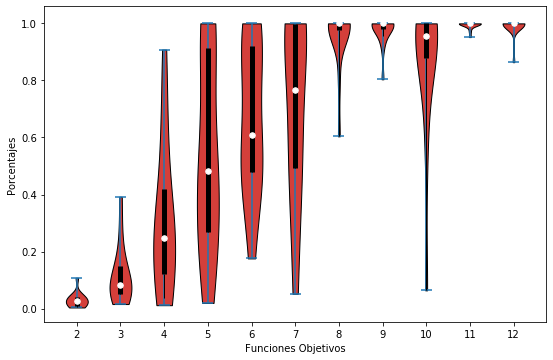
\includegraphics[width=0.7\linewidth]{fobjetivos.png}
	    	\caption{Diagrama de Violín y de Caja Bigote.}
	    	\label{fig:imagen3}
	    		\newpage
	    	
	    	\end{figure}
    	
 
    \section{Conclusiones}
    Tomando como referencia los resultados mostrados en el diagrama, y la tabla de resultados se concluye lo siguiente:
    \begin{enumerate}			
    	\item	Entre más objetivos haya, se tienen mayor cantidad de soluciones no dominadas. Lo anterior, lo podemos interpretar de la siguiente manera: entre más objetivos existan, las soluciones tienden tener mayor dominancia. 
    	\item	La conclusión de los resultados que se obtuvieron indica que ante mayor cantidad de objetivos, tenemos mayor complejidad para poder elegir una solución no dominada  ya que tenemos demasiadas posibilidades de selección.  
    	
    \end{enumerate}

\bibliography{Biblio}
\bibliographystyle{plainnat}

    
\end{document}